\section{Definición de componentes comunes}
\label{sub:componentes_comunes}

En esta sección se pretende ubicar a los bloques que hacen a la base del
lenguaje, cuestiones que se utilizan como herramientas para definir otros
componentes más complejos.

Dado lo básico de los componentes aquí presentados no se adjuntarán Autómatas
Finitos ni tampoco Árboles Sintácticos para los mismos.

\subsection{letra}
\label{sub:letra}

\subsubsection{Analizador Léxico}

Para un patrón de expresiones regulares se tiene lo
siguiente con respecto a las letras:

\begin{lstlisting}[basicstyle=\footnotesize\ttfamily, caption={Regex - letra}]
Regex: /[a-zA-Z]?/
\end{lstlisting}

\subsubsection{Analizador Sintáctico}

Segun la notación BNF se tiene lo siguiente:

\begin{lstlisting} [basicstyle=\footnotesize\ttfamily, caption={BNF - letra}]
	<letra> ::= "a" | "b" | "c" | "d" | "e" | "f" | "g" | "h" | "i" |
	            "j" | "k" |	"l" | "m" | "n" | "o" | "p" | "q" | "r" |
							"s" | "t" | "u" | "v" | "w" | "x" | "y" |	"z" | "A" |
							"B" |	"C" | "D" | "E" | "F" | "G" | "H" | "I" | "J" |
							"K" | "L" | "M" |	"N" | "O" | "P" |	"Q" | "R" | "S" |
							"T" |	"U" | "V" | "W" | "X" | "Y" | "Z"
\end{lstlisting}


\subsection{digito}
\label{sub:digito}

\subsubsection{Analizador Léxico}

En cuanto a la expresión regular para los mismos se define de la siguiente
manera:

\begin{lstlisting}[basicstyle=\footnotesize\ttfamily]
	Regex: /[0-9]/
\end{lstlisting}

\subsubsection{Analizador Sintáctico}

La notación para la gramática libre de contexto en formato BNF para los
\texttt{dígitos} es la siguiente:

\begin{lstlisting}[basicstyle=\footnotesize\ttfamily, caption={BNF - digito}]
  <digito> ::= "0"|"1"|"2"|"3"|"4"|"5"|"6"|"7"|"8"|"9"
\end{lstlisting}

\subsection{simbolo}
\label{sub:simbolo}

\subsubsection{Analizador Léxico}

Expresión regular para la descripción de los símbolos:

\begin{lstlisting}[basicstyle=\footnotesize\ttfamily, caption={Regex - simbolo}]
  Regex: /\W|_/
\end{lstlisting}

\subsubsection{Analizador Sintáctico}

BNF para describir un símbolo dentro del lenguaje se expone a continuación:

\begin{lstlisting}[basicstyle=\footnotesize\ttfamily, caption={BNF - simbolo}]
	<simbolo> ::= "|" | " " | "!" | "#" | "$" | "%" | "&" | "(" | ")"
	              | "*" | "+"	| "," | "-" | "." | "/" | ":" | ";"
								| ">" | "=" | "<"	| "?" | "@" | "[" | "\"	| "]"
								| "^" | "_" | "`" | "{" | "}" | "~"
\end{lstlisting}


\subsection{texto}
\label{sub:texto}
La definición de este elemento simplifica futuro manejo de cuestiones dentro de
la definición del lenguaje, el elemento \texttt{texto} es la aplicación
sucesiva de los elementos \texttt{letra}, \texttt{digito} y \texttt{simbolo}.

\subsubsection{Analizador Léxico}

El autómata finito para este explica al relación de los tres elementos
mencionados:

\begin{figure}[H]
	\centering
	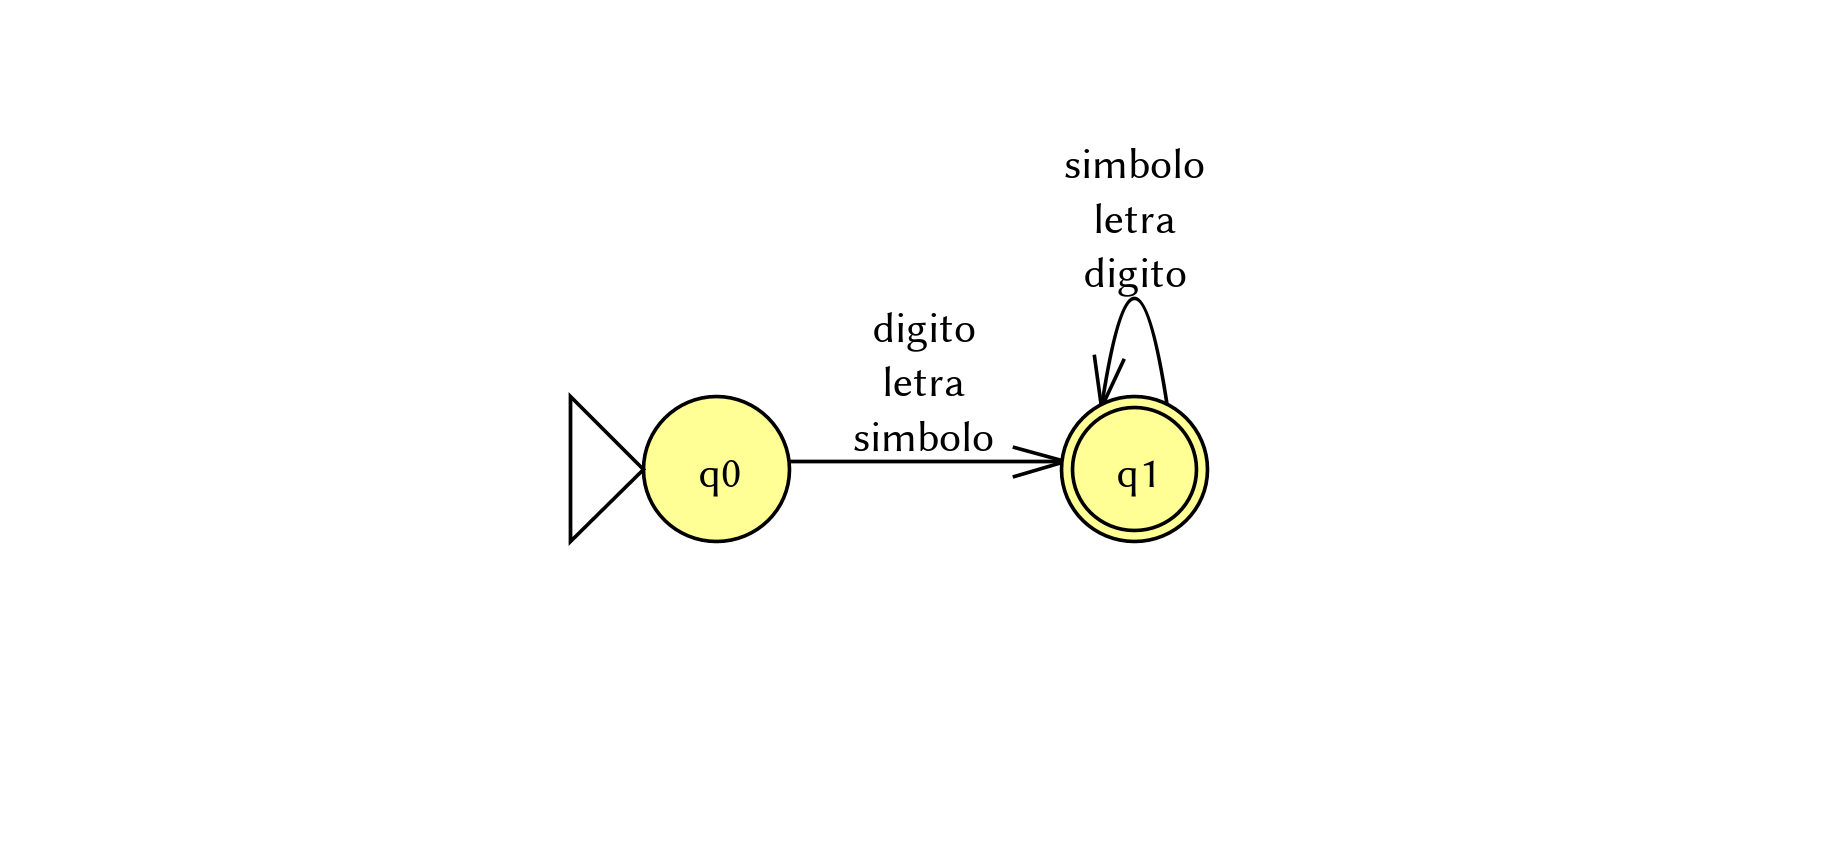
\includegraphics[width=.7\linewidth]{automatas_finitos/textoDrt.png}
	\caption{Autómata finito - texto}
	\label{fig:texto}
\end{figure}

en cuanto a la expresion regular se puede definir de la siguiente manera:

\begin{lstlisting}[basicstyle=\footnotesize\ttfamily, caption={Regex - texto}]
  Regex: / [a-zA-z_]|[0-9]|\W /
\end{lstlisting}

\subsubsection{Analizador Sintáctico}

El BNF para el elemento se describe de la siguiente manera:

\begin{lstlisting}[basicstyle=\footnotesize\ttfamily, caption={BNF - texto}]
  <texto> ::= <letra|digito|simbolo> <texto>
\end{lstlisting}

\subsection{nombre}
\label{sub:nombre}
Esta expresión se utiliza a lo largo del documento para hacer referencia a
cadenas de texto que identifiquen un elemento del lenguaje, como por ejemplo,
utilizando con la palabra \texttt{class} este pasaría a definir el nombre de la
clase, si se utiliza con en un contexto de atributo, este sería
el nombre que identifica a ese atributo. A continuación, se presenta la
gramática libre de contexto y la expresión regular para un elemento
\texttt{nombre} dentro del lenguaje, antes, se crea una herramienta que permita el uso
recursivo de \texttt{letra}, \texttt{simbolo} y \texttt{digito}.
Si bien esto se parece bastante a lo que se expone en la \texttt{Subsección
\ref{sub:texto}} per se tiene la necesidad de restringir el uso de símbolos
a únicamente el uso del guión bajo ``\_''.

\subsubsection{Analizador Léxico}

\begin{lstlisting}[basicstyle=\footnotesize\ttfamily, caption={Regex - nombre}]
  Regex: /[a-zA-Z][a-zA-Z_][0-9]*/
\end{lstlisting}

El autómata finito para esta expresion es el siguiente:

\begin{figure}[H]
	\centering
	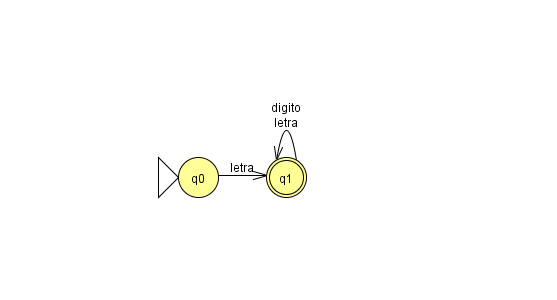
\includegraphics[width=.7\linewidth]{automatas_finitos/nombreDrt.png}
	\caption{Autómata finito - nombre}
	\label{fig:nombre}
\end{figure}

\subsubsection{Analizador Sintáctico}

\begin{lstlisting}[basicstyle=\footnotesize\ttfamily]
  <nombre-texto> ::= <letra|digito|"_"> <nombre-texto>
\end{lstlisting}

\begin{lstlisting}[basicstyle=\footnotesize\ttfamily, caption={BNF - nombre}]
  <nombre> ::= <letra> <nombre-texto>
\end{lstlisting}


\subsection{visibilidad}
\label{sub:visibilidad}
La visibilidad, como ya se explicó implícitamente en la descripción de algunas
de las palabras reservadas expuestas en la \texttt{Sección
\ref{sec:palabrasreservadas}}, tiene la función de establecer que miembros del
modelo tienen acceso ciertos elementos, el hecho de que estas estén compuestas
de palabras reservadas hace que su generalización con componentes de más bajo
nivel descritos en las \texttt{Secciones \ref{sub:letra}},
\texttt{\ref{sub:digito}} y \texttt{\ref{sub:nombre}} no sea posible, por esta
razón se hace la descripción con los componentes literales que hacen a la
visibilidad.

\subsubsection{Analizador Léxico}
Se presenta la expresión regular correspondiente a lo descrito
anteriormente:

\begin{lstlisting}[language=Java, basicstyle=\footnotesize\ttfamily]
	Regex: /(public|+|private|-|protected|#|derivate|/|package|~)/
\end{lstlisting}

dada la simpleza de la expresión regular no se brinda el Autómata para el
mismo.

\subsubsection{Analizador Sintáctico}
La notación BNF para la visibilidad es como se expone a continuación:

\begin{lstlisting}[basicstyle=\footnotesize\ttfamily, caption={BNF -
visibilidad (v1)}]
  <visibilidad> ::= public | private | protected | derivate | package
\end{lstlisting}

Si bien esto permite describir la visibilidad de los componentes del modelo,
según la especificación UML, en su totalidad, en el apartado
\ref{sec:simbolosespeciales} expone que el lenguaje preserva la naturaleza
gráfica de UML permitiendo que el usuario utilice símbolos para la definición
de visibilidad en diferentes componentes de un modelo, por lo tanto, teniendo
esto en consideración, la nueva expresión BNF para la \texttt{visibilidad} es
como sigue:

\begin{lstlisting}[language=Java, basicstyle=\footnotesize\ttfamily,
caption={BNF - visibilidad (final)}]
  <visibilidad> ::= public | + | private | - | protected | # |
	                  derivate | / | package | ~
\end{lstlisting}

\subsection{tipo}
\label{sub:tipo}
Este componente permite identificar la naturaleza de métodos y atributos dentro
de un modelo, estos, al igual que los componentes de la \texttt{visibilidad}
explicados en la \texttt{Subsección \ref{sub:visibilidad}}, están basados en
literales que forman parte del conjunto de palabras reservadas del lenguaje,
esta es la razón por la cual el \texttt{tipo} tampoco se puede generalizar como
también es mencionado en la subsección anterior.

El tipo se puede describir de la siguiente manera:

\subsubsection{Analizador Léxico}

en cuanto a la expresión regular que concierne a la gramática anterior se
describe a continuación como:

\begin{lstlisting}[basicstyle=\footnotesize\ttfamily]
	Regex: /(integer|double|float|long|boolean|string|char)/
\end{lstlisting}


\subsubsection{Analizador Sintáctico}

\begin{lstlisting}[basicstyle=\footnotesize\ttfamily]
	<tipo> ::= integer | double | float | long | boolean |
	           string | char
\end{lstlisting}

